\documentclass[11pt,twoside]{article}
\usepackage[french]{babel}
\usepackage{libertine}
\usepackage{listings}
\usepackage{graphicx}
\usepackage[T1]{fontenc}
\usepackage[utf8]{inputenc}
\usepackage[a4paper]{geometry}
\geometry{verbose,lmargin=4.5cm,rmargin=3.4cm}
\usepackage{color}
\usepackage{babel}
\usepackage{refstyle}
\usepackage{algorithm2e}
\usepackage{microtype}
\usepackage{fancyhdr}
\usepackage{lettrine}
\usepackage[unicode=true,pdfusetitle,
 bookmarks=true,bookmarksnumbered=true,bookmarksopen=false,
 breaklinks=true,pdfborder={0 0 0},pdfborderstyle={},backref=section,colorlinks=true]
 {hyperref}
\hypersetup{
 pdfsubject={Un assembleur et VM pour les étudiants, par des étudiants},
 pdfkeywords={asm,assembleur,vm}}

\renewcommand*\familydefault{\sfdefault}

\makeatletter
\addto\extrasfrench{%
   \providecommand{\og}{\leavevmode\flqq~}%
   \providecommand{\fg}{\ifdim\lastskip>\z@\unskip\fi~\frqq}%
}

\makeatletter
\newcommand{\noun}[1]{\textsc{#1}}
\makeatother

\setlength{\headheight}{15pt}
\pagestyle{fancy}
\fancyhead[LE,RO]{\noun{Eva}}
\fancyhead[C]{}
\fancyfoot[C]{}
\fancyfoot[LO, RE]{\noun{CodeAnon}}
\fancyfoot[RO,LE]{\thepage}

\begin{document}
\title{EVA}
\author{Association CodeAnon}

\maketitle
\begin{abstract}
  Nous proposons une machine virtuelle destinée aux étudiants, concue et implantée par des étudiants, afin de faciliter l'apprentissage de la programmation bas niveau. La machine virtuelle, bien que simple, reste complète, permettant aux utilisateurs de faire tourner des programmes complets avec \noun{Eva}.
\end{abstract}
\vfill
\begin{center}
  
\includegraphics[height=8cm]{logo_graph.pdf}
\end{center}
\vfill
\cleardoublepage

\hspace{0pt}
\vfill

\section*{Remarque préliminaire}

Ce document est écrit au présent. Il n'en reste pas moins une projection de ce que sera \noun{Eva} au terme de son développement. Il faut donc le lire comme une description détaillée du projet final \noun{Eva} et non comme une description de son état actuel. Par ailleurs des modifications seront certainement apportées à ce document durant le développement d'\noun{Eva}.

\vfill
\hspace{0pt}

\clearpage

\tableofcontents
\cleardoublepage

\hspace{0pt}
\vfill

\section{Introduction}

\lettrine[lines=3,slope=.3em]%
{L}{e} langage assembleur constitue la première abstraction à la programmation
de circuits programmables. Aussi son apprentissage est une étape fondamentale pour l'étudiant curieux de comprendre le fonctionnement des ordinateurs. Mais d'autres applications nécessitent une bonne connaissance des langages d'assemblage. L'écriture des compilateurs par exemple repose assez largement sur une connaissance fine des différentes architectures existantes (ARM, elf, x86 ...) et des langages d'assemblage qui leurs sont associés.

Comment alors permettre aux étudiants désireux de s'initier à l'écriture de compilateur ou d'applications très bas niveau de réaliser leurs projets ? Face à l'étendue des architectures à cibler, à la complexité de certaines d’entre elles, ce type de projet peut rapidement devenir compliqué. Bien sur, des alternatives existent déjà. On peut citer le fameux ouvrage \textit{Structure And interpretation of Computer Programs} \cite{SICP} qui propose en dernier chapitre l'implémentation d'une machine abstraite programmable dans un langage d'assemblage simple. D'autres projets comme la machine virtuelle CHIP8 sont des sources intéressantes pour découvrir la programmation assembleur \cite{CHIP8}. Ces outils déjà utilisés dans le but de rendre accessible aux étudiants les thématiques dites de \og~bas niveaux\fg restent néanmoins très spécifiques et limitent grandement le champs des possibles. C'est à ce carrefour entre facilité d'apprentissage et possibilités offertes; ce delta entre outil pédagogique et problèmes en tailles réelles qu'essaye de s'intercaler le projet \noun{Eva}. \\

\section{Projets existants}

D'autres machines virtuelles existent, telles que la JVM (\emph{Java Virtual Machine}) où le CLR (\emph{Common Language Runtime}), qui sont destinés à un usage généraliste. Ces machines virtuelles sont performantes, optimisées et complètes; cependant ceci rend ces projets inatteignables pour des étudiants en license, même informatique.\\
D'autres VMs comme le CHIP8 sont trop limités, et perdent le côté utilisable; ces machines sont faciles à raisonner et à implanter mais de par leur simplicité il est impossible de programmer des programmes de complexité grandissante.

\vfill
\hspace{0pt}
\newpage{}

\section{Description du projet}

\noun{Eva} est une machine virtuelle développée par des étudiants pour les
étudiants. Simple et légère, elle offre un terrain d'expérimentation
particulièrement adapté à l'apprentissage de l'assembleur ou encore
à l'écriture de compilateurs. Son code source publique, clair et documenté
la rendent accessible et facilement modifiable. \noun{Eva} est programmable
dans un langage assembleur dédié facile d'accès et doté d'un jeu d'instructions
succinct mais complet. Par complet nous entendons informellement ``suffisant pour permettre d'implanter une application incluant des entrées, des sorties et éventuellement des fonctions de réseaux ou d'affichage graphique''. Nous reviendrons en détail sur ce point dans la suite du document.

\section{Description technique}

L'ensemble du projet \noun{Eva} se compose de plusieurs outils \figref{diagram1}.

\begin{itemize}
  \item \textbf{Cœur de la VM} \\
        Il s'agit d'un interpréteur pour le langage machine de \noun{Eva}. C'est ce programme qui fait l'interface entre l'utilisateur de \noun{Eva} et sa machine.

  \item \textbf{Assembleur Eva} \\
        Ce dernier permet la conversion d'un code assembleur en un fichier exécutable par la VM. Il est également accompagné d'un éditeur de lien permettant de composer des exécutables à partir de plusieurs modules assembleur.

  \item \textbf{Outil de débogage} \\
        Cet outil permet aux utilisateurs de lancer l’exécution de leurs programmes en mode pas à pas. Ils peuvent ainsi observer en détail le comportement de leurs programmes et comment la VM les traite. On peut par ce biais contrôler le contenu de la mémoire et des registres de la VM.


  \item \textbf{Bibliothèque Standard} \\
        Le projet \noun{Eva} est livré avec une collection de modules utilitaires. Il peut s'agir par exemple de fonctions d'affichage ou de calcul mathématique. Cette bibliothèque peut être explicitement chargée en mémoire avant le lancement de la VM, on pourra alors l'utiliser via des \og~appels systèmes\fg. Une autre alternative étant de passer par une étape d'édition de lien pour embarquer une sélection de module dans un exécutable.

\end{itemize}

\begin{figure}[tb]
  \centering
  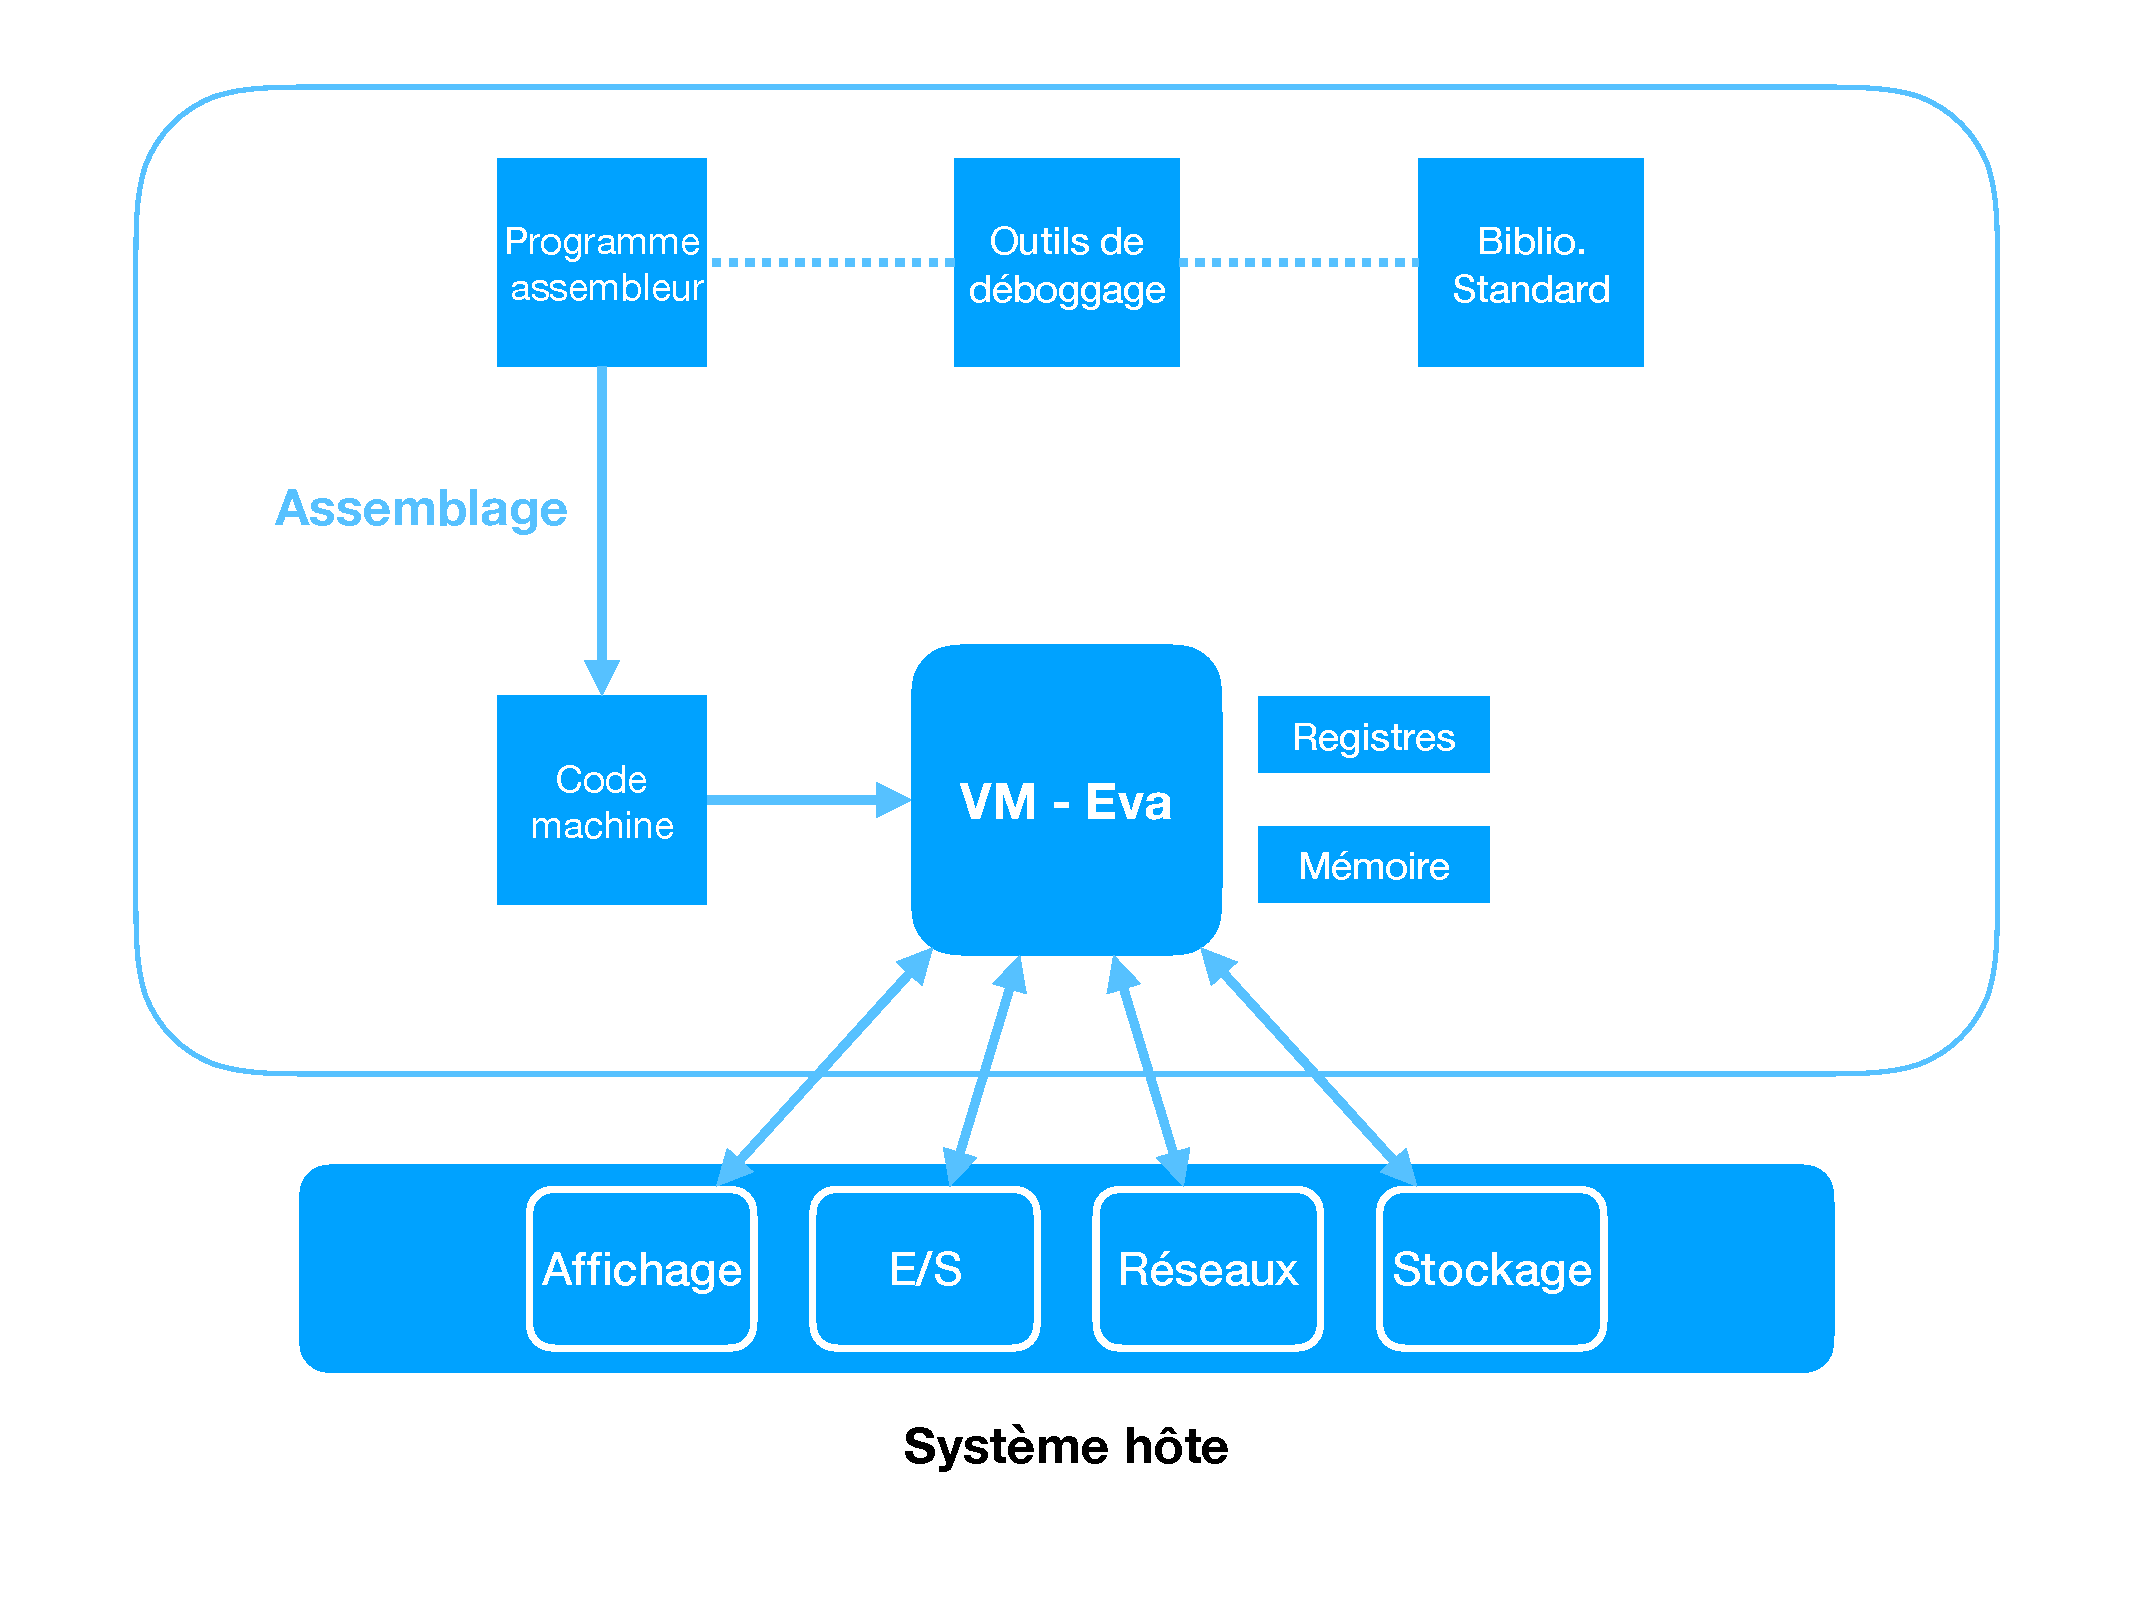
\includegraphics[width=12cm, height=12cm, keepaspectratio]{diagram1_graph.pdf}
  \caption{Structure de la machine virtuelle \noun{Eva}}
  \label{fig:diagram1}
\end{figure}


\section{Éléments de conception}

La machine virtuelle doit être minimaliste pour que la compréhension de son fonctionnement soit accessible, simple à programmer pour rester accessible aux étudiants désireux d'apprendre, mais également suffisamment performante pour supporter le développement d'applications en vrai grandeur. \noun{Eva} étant conçue sur la base du \og retour aux fondamentaux\fg , elle va donc à l'essentiel et propose un jeu d'instructions à la fois concis et simple à prendre en main sans fonctionnalités superflue. Nous avons à ces fins sélectionné un sous-ensemble des instructions ARM \tabref{instructions}.

\begin{table}[tb]
  \begin{centering}
    \begin{tabular}{|c|l|}
      \hline
      \textbf{Instruction} & \textbf{Description}                \\
      \hline
      \hline
      \textbf{ADD}         & Addition                            \\
      \hline
      \textbf{ADC}         & Addition avec retenue               \\
      \hline
      \textbf{BIC}         & RAZ de bit                          \\
      \hline
      \textbf{CMP}         & Comparaison                         \\
      \hline
      \textbf{MOV}         & Écriture de valeur dans le registre \\
      \hline
      \textbf{B}           & \emph{Branch Jump}                  \\
      \hline
      \textbf{BL}          & \emph{Branch Link}                  \\
      \hline
      \textbf{PUSH}        & Empiler                             \\
      \hline
      \textbf{POP}         & Dépiler                             \\
      \hline
      \textbf{SUB}         & Soustraction avec retenue           \\
      \hline
    \end{tabular}
    \par\end{centering}
  \caption{Liste des instructions de la machine virtuelle d'\noun{Eva}.}
  \label{tab:instructions}
\end{table}


\section{Implantation de la machine virtuelle}

Afin d'aider au développement du projet, \noun{Eva} va être implantée
en C (norme 99) et ne doit dépendre d'aucun code source autre que
la librairie standard. Une telle contrainte assure que l'implantation
soit claire, le code source portable, et la compilation aisée.

Cette implantation minimale va de paire avec l'idéologie derrière
\noun{Eva} : prioriser l'accessibilité et la fiabilité. De plus, l'aspect
sécurité est d'une grande importance pour le projet et la correction
du code aura toujours priorité sur l'ajout de nouvelles fonctionnalités.

\section{Disponibilité du projet}

\noun{Eva} est un projet publique, dont le code et les binaires seront
accessibles en open-source, suivant une licence MIT. Cela veut dire
que n'importe quel utilisateur peut télécharger, lire et modifier
le code source. Le projet étant pédagogique, il va de soit que chaque
composante du projet soit publique et accessible pour le plus grand nombre.

\section{Projets connexes}

En plus du développement de la machine virtuelle, \noun{Eva} sera
également le socle de plusieurs projets dont divers compilateurs ciblant
\noun{Eva}. Parmi ces compilateurs l'équipe d'\noun{Eva} développera et maintiendra
un langage de programmation de haut niveau spécifique à \noun{Eva}. Ce dernier
permettra de complémenter les possibilités offertes par le simple langage
assembleur supporté nativement par la plate-forme.

\section{Exemples d’utilisation}

Dans cette section nous présentons rapidement quelques scénarios classique d'utilisation d'\noun{Eva}.

\begin{itemize}
  \item \textbf{Assemblage d'un fichier} \\
        \lstinline$evasm -a source.evasm -o main.evo$

  \item \textbf{Assemblage et édition directe d'un fichier unique} \\
        \lstinline$evasm source.evasm -o main.eva$

  \item \textbf{Édition d'un ensemble de modules} \\
        \lstinline$evasm -l module1.evo module2.evo source.evo -o main.eva$

  \item \textbf{Exécution d'un fichier} \\
        \lstinline$eva main.eva$

  \item \textbf{Exécution d'un fichier avec débogage} \\
        \lstinline$eva main.eva --debug$

  \item \textbf{Exécution d'un fichier avec limitation de mémoire utilisées (en mo)} \\
        \lstinline$eva main.eva --ram 200$

  \item \textbf{Exécution d'un fichier avec chargement explicite de la bibliothèque standard} \\
        \lstinline$eva main.eva --std$
\end{itemize}


\newpage{}

\clearpage{}

\begin{thebibliography}{XXXXXX}
  \label{chap:bib}

  \bibitem{SICP} Harold Abelson and Gerald Jay Sussman
  \emph{Structure and Interpretation of Computer Programs} MIT, 1996

  \bibitem{CHIP8} Joseph Weisbecker
  \emph{CHIP-8 programming language and virtual machine} 1978

\end{thebibliography}

\end{document}
